\documentclass{standalone}%
\usepackage[T1]{fontenc}%
\usepackage[utf8]{inputenc}%
\usepackage{lmodern}%
\usepackage{textcomp}%
\usepackage{lastpage}%
\usepackage{tikz}%
\usetikzlibrary{decorations.pathreplacing,calligraphy}
%
%
%
\begin{document}%
\normalsize%
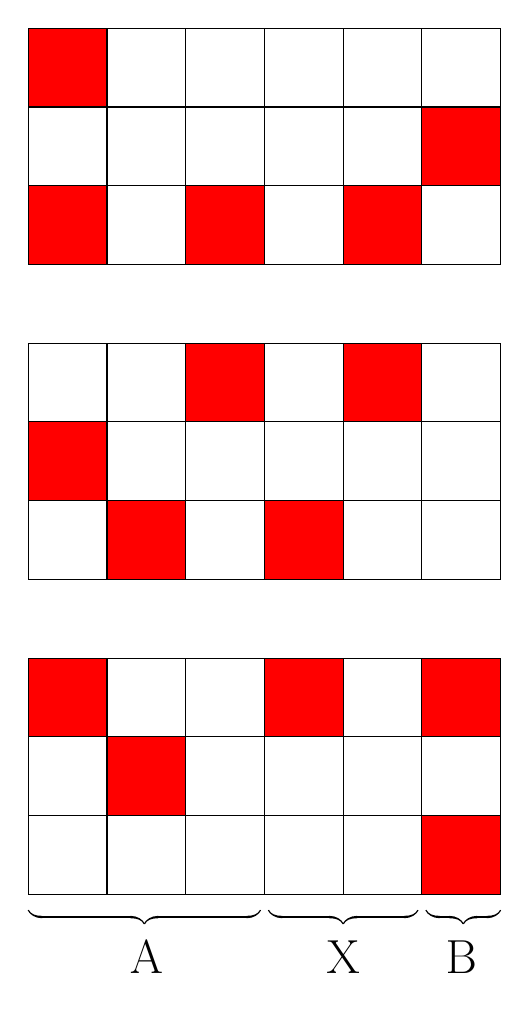
\begin{tikzpicture}[scale=1.0]%
\path[draw,draw] (0.0,0.0) rectangle (1.0,1.0);%
\path[draw,draw] (1.0,0.0) rectangle (2.0,1.0);%
\path[draw,draw] (2.0,0.0) rectangle (3.0,1.0);%
\path[draw,draw] (3.0,0.0) rectangle (4.0,1.0);%
\path[draw,draw] (4.0,0.0) rectangle (5.0,1.0);%
\path[draw,draw] (5.0,0.0) rectangle (6.0,1.0);%
\path[draw,draw] (0.0,-1.0) rectangle (1.0,0.0);%
\path[draw,draw] (1.0,-1.0) rectangle (2.0,0.0);%
\path[draw,draw] (2.0,-1.0) rectangle (3.0,0.0);%
\path[draw,draw] (3.0,-1.0) rectangle (4.0,0.0);%
\path[draw,draw] (4.0,-1.0) rectangle (5.0,0.0);%
\path[draw,draw] (5.0,-1.0) rectangle (6.0,0.0);%
\path[draw,draw] (0.0,-2.0) rectangle (1.0,-1.0);%
\path[draw,draw] (1.0,-2.0) rectangle (2.0,-1.0);%
\path[draw,draw] (2.0,-2.0) rectangle (3.0,-1.0);%
\path[draw,draw] (3.0,-2.0) rectangle (4.0,-1.0);%
\path[draw,draw] (4.0,-2.0) rectangle (5.0,-1.0);%
\path[draw,draw] (5.0,-2.0) rectangle (6.0,-1.0);%
\path[draw,draw] (0.0,-4.0) rectangle (1.0,-3.0);%
\path[draw,draw] (1.0,-4.0) rectangle (2.0,-3.0);%
\path[draw,draw] (2.0,-4.0) rectangle (3.0,-3.0);%
\path[draw,draw] (3.0,-4.0) rectangle (4.0,-3.0);%
\path[draw,draw] (4.0,-4.0) rectangle (5.0,-3.0);%
\path[draw,draw] (5.0,-4.0) rectangle (6.0,-3.0);%
\path[draw,draw] (0.0,-5.0) rectangle (1.0,-4.0);%
\path[draw,draw] (1.0,-5.0) rectangle (2.0,-4.0);%
\path[draw,draw] (2.0,-5.0) rectangle (3.0,-4.0);%
\path[draw,draw] (3.0,-5.0) rectangle (4.0,-4.0);%
\path[draw,draw] (4.0,-5.0) rectangle (5.0,-4.0);%
\path[draw,draw] (5.0,-5.0) rectangle (6.0,-4.0);%
\path[draw,draw] (0.0,-6.0) rectangle (1.0,-5.0);%
\path[draw,draw] (1.0,-6.0) rectangle (2.0,-5.0);%
\path[draw,draw] (2.0,-6.0) rectangle (3.0,-5.0);%
\path[draw,draw] (3.0,-6.0) rectangle (4.0,-5.0);%
\path[draw,draw] (4.0,-6.0) rectangle (5.0,-5.0);%
\path[draw,draw] (5.0,-6.0) rectangle (6.0,-5.0);%
\path[draw,draw] (0.0,-8.0) rectangle (1.0,-7.0);%
\path[draw,draw] (1.0,-8.0) rectangle (2.0,-7.0);%
\path[draw,draw] (2.0,-8.0) rectangle (3.0,-7.0);%
\path[draw,draw] (3.0,-8.0) rectangle (4.0,-7.0);%
\path[draw,draw] (4.0,-8.0) rectangle (5.0,-7.0);%
\path[draw,draw] (5.0,-8.0) rectangle (6.0,-7.0);%
\path[draw,draw] (0.0,-9.0) rectangle (1.0,-8.0);%
\path[draw,draw] (1.0,-9.0) rectangle (2.0,-8.0);%
\path[draw,draw] (2.0,-9.0) rectangle (3.0,-8.0);%
\path[draw,draw] (3.0,-9.0) rectangle (4.0,-8.0);%
\path[draw,draw] (4.0,-9.0) rectangle (5.0,-8.0);%
\path[draw,draw] (5.0,-9.0) rectangle (6.0,-8.0);%
\path[draw,draw] (0.0,-10.0) rectangle (1.0,-9.0);%
\path[draw,draw] (1.0,-10.0) rectangle (2.0,-9.0);%
\path[draw,draw] (2.0,-10.0) rectangle (3.0,-9.0);%
\path[draw,draw] (3.0,-10.0) rectangle (4.0,-9.0);%
\path[draw,draw] (4.0,-10.0) rectangle (5.0,-9.0);%
\path[draw,draw] (5.0,-10.0) rectangle (6.0,-9.0);%
\path[draw,draw,fill=red] (0.0,0.0) rectangle (1.0,1.0);%
\path[draw,draw,fill=red] (5.0,-1.0) rectangle (6.0,0.0);%
\path[draw,draw,fill=red] (0.0,-2.0) rectangle (1.0,-1.0);%
\path[draw,draw,fill=red] (2.0,-2.0) rectangle (3.0,-1.0);%
\path[draw,draw,fill=red] (4.0,-2.0) rectangle (5.0,-1.0);%
\path[draw,draw,fill=red] (2.0,-4.0) rectangle (3.0,-3.0);%
\path[draw,draw,fill=red] (4.0,-4.0) rectangle (5.0,-3.0);%
\path[draw,draw,fill=red] (0.0,-5.0) rectangle (1.0,-4.0);%
\path[draw,draw,fill=red] (1.0,-6.0) rectangle (2.0,-5.0);%
\path[draw,draw,fill=red] (3.0,-6.0) rectangle (4.0,-5.0);%
\path[draw,draw,fill=red] (0.0,-8.0) rectangle (1.0,-7.0);%
\path[draw,draw,fill=red] (3.0,-8.0) rectangle (4.0,-7.0);%
\path[draw,draw,fill=red] (5.0,-8.0) rectangle (6.0,-7.0);%
\path[draw,draw,fill=red] (1.0,-9.0) rectangle (2.0,-8.0);%
\path[draw,draw,fill=red] (5.0,-10.0) rectangle (6.0,-9.0);%


\draw[decorate, decoration={calligraphic brace, mirror, amplitude=5pt}, line width=0.3mm] (0,-10.2) -- (2.95,-10.2);
\node at (1.5,-10.8) {\LARGE A};

\draw[decorate, decoration={calligraphic brace, mirror, amplitude=5pt}, line width=0.3mm] (3.05,-10.2) -- (4.95,-10.2);
\node at (4,-10.8) {\LARGE X};

\draw[decorate, decoration={calligraphic brace, mirror, amplitude=5pt}, line width=0.3mm] (5.05,-10.2) -- (6,-10.2);
\node at (5.5,-10.8) {\LARGE B};
\end{tikzpicture}%
\end{document}